\documentclass[10pt]{article}

\usepackage{mathtools}
\DeclarePairedDelimiter\ceil{\lceil}{\rceil}
\DeclarePairedDelimiter\floor{\lfloor}{\rfloor}

%\usepackage{algpseudocode}
\usepackage{graphicx}
\graphicspath{{img/}}
\usepackage{amsmath}
\usepackage[margin=1.0in]{geometry}
\usepackage{hyperref}
\hypersetup{
	colorlinks=true,
	linkcolor=blue
}


\begin{document}

\title{\vspace{-2.0cm}Project 3A: Image Mosaic}
\author{Taylor Nelms and Nikhil Shenoy}
\date{\today}

\maketitle

\section{How to Run}
	You can run this project by executing ``python mymosaic.py'' from the command line with options that specify the images to be stitched. To do a nearest neighbors calculation, we used the KDTree from scipy.spatial. We use the ``argparse`` module to handle various inputs. These are the available options:

	\begin{itemize}
		\item \textbf{-l}: Specify the path to the left image.
		\item \textbf{-m}: Specify the path to the middle image.
		\item \textbf{-r}: Specify the path to the right image.
	\end{itemize}

	Please note that this project works for stitching strictly three images together.

\section{Potential Packages to Install}

	\begin{itemize}
		\item argparse
		\item scipy
	\end{itemize}

\section{Image Outputs}

	\subsection{Classroom}
		\begin{figure}[h]
			\caption{ANMS for the left image}
			\centering
			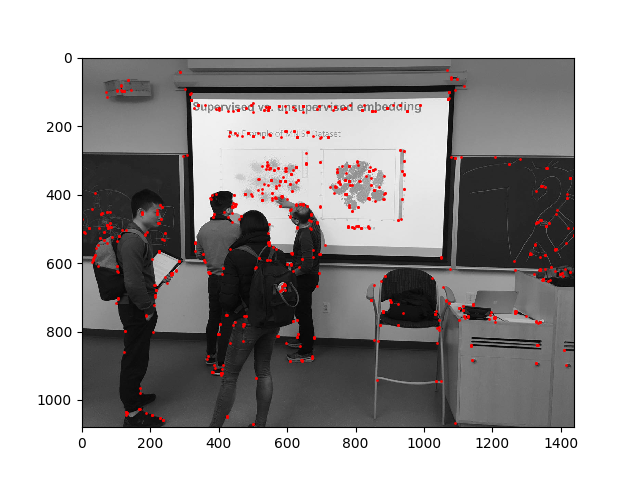
\includegraphics{img/anmsL.png}
		\end{figure}
		
		\begin{figure}[h]
			\caption{ANMS for the middle image}
			\centering
			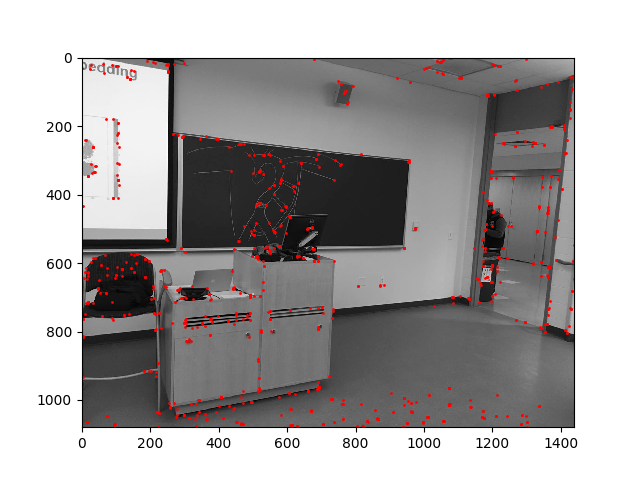
\includegraphics{img/anmsM.png}
		\end{figure}

			\begin{figure}[h]
			\caption{ANMS for the right image}
			\centering
			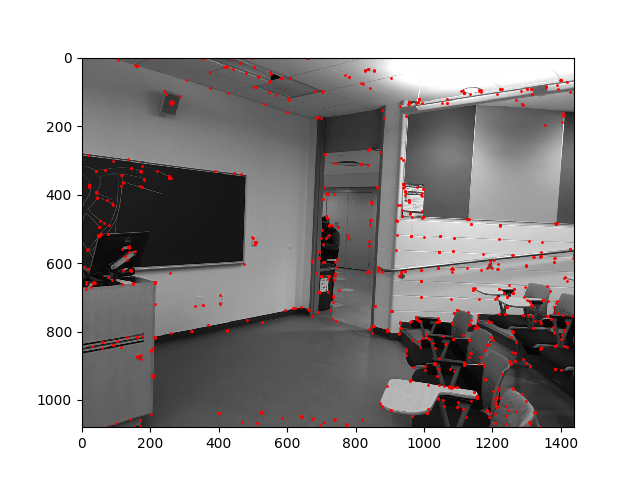
\includegraphics{img/anmsR.png}
		\end{figure}
			
		\begin{figure}[h]
			\caption{Post-RANSAC points using the left and middle images}
			\centering
			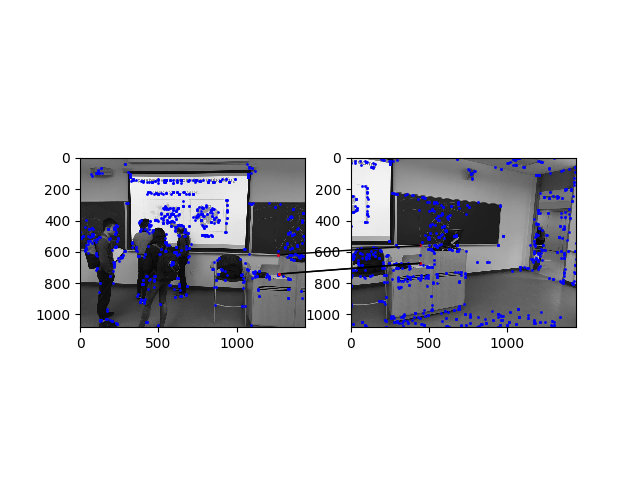
\includegraphics{img/postranLM.png}
		\end{figure}
		
		\begin{figure}[h]
			\caption{Post-RANSAC points using the middle and right images}
			\centering
			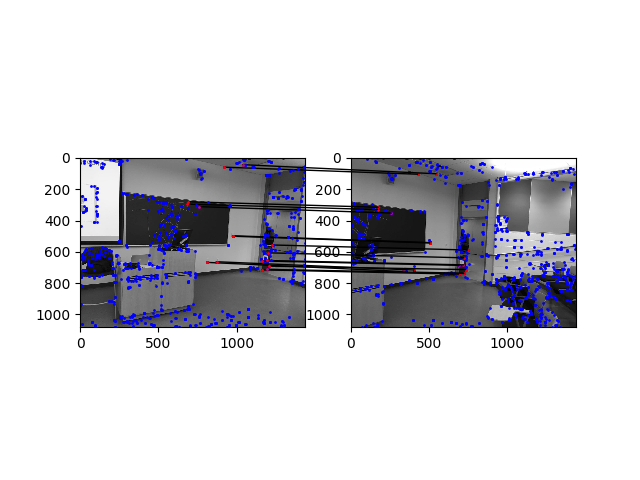
\includegraphics{img/postranMR.png}
		\end{figure}
		

		\begin{figure}[h]
			\caption{Final panorama}
			\centering
			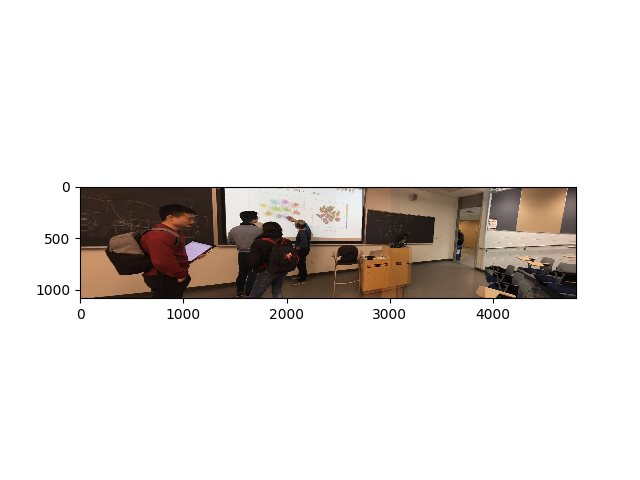
\includegraphics{img/mosaic.png}
		\end{figure}

	\subsection{Street}
		\begin{figure}[h]
			\caption{ANMS for the left image}
			\centering
			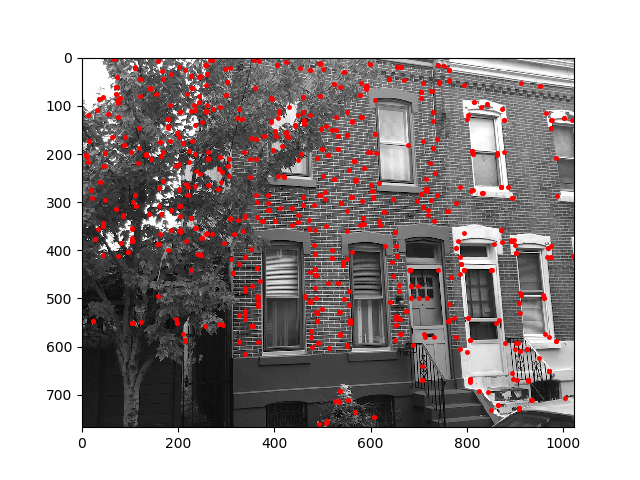
\includegraphics{img/bricksANMSleft.png}
		\end{figure}
		
		\begin{figure}[h]
			\caption{ANMS for the middle image}
			\centering
			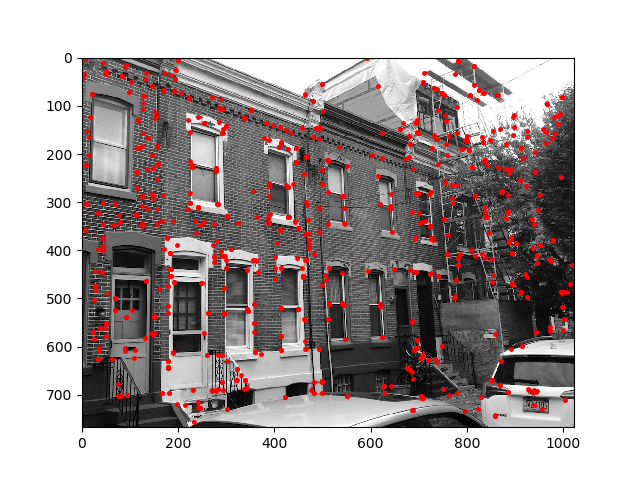
\includegraphics{img/bricksANMSmiddle.png}
		\end{figure}

			\begin{figure}[h]
			\caption{ANMS for the right image}
			\centering
			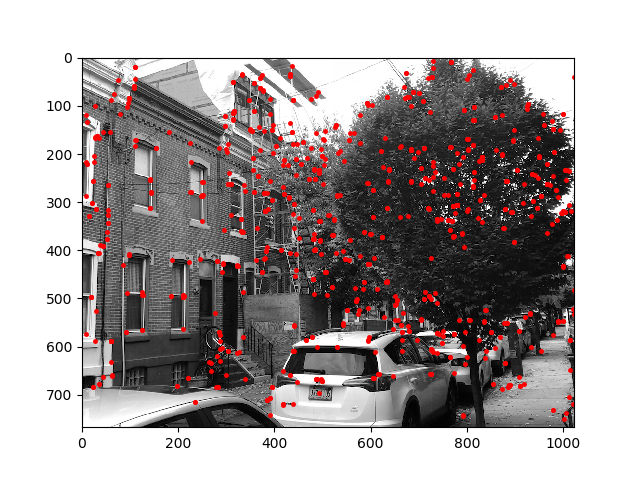
\includegraphics{img/bricksANMSright.png}
		\end{figure}
			
		\begin{figure}[h]
			\caption{Post-RANSAC points using the left and middle images}
			\centering
			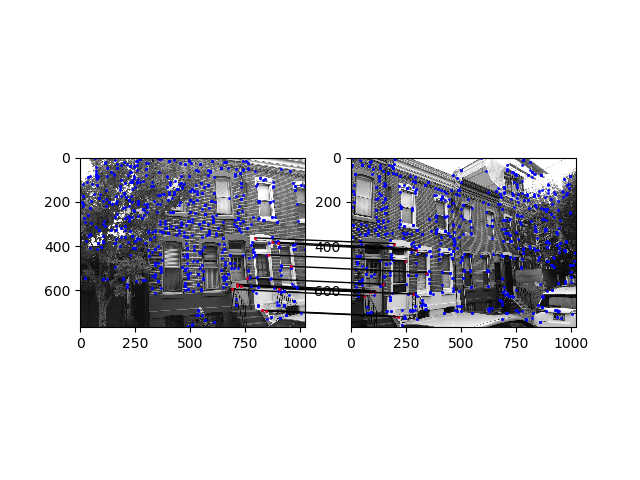
\includegraphics{img/bricksRANSACl2m.png}
		\end{figure}
		
		\begin{figure}[h]
			\caption{Post-RANSAC points using the middle and right images}
			\centering
			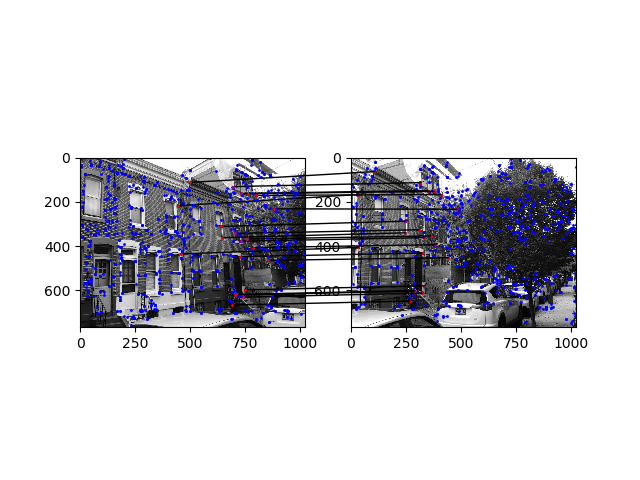
\includegraphics{img/bricksRANSACm2r.png}
		\end{figure}
		

		\begin{figure}[h]
			\caption{Final panorama}
			\centering
			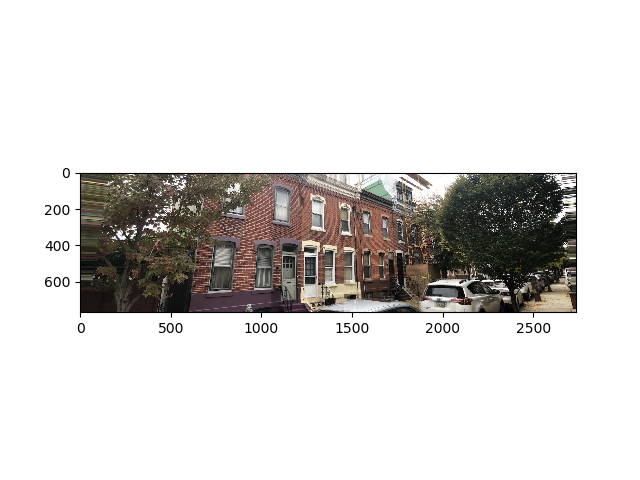
\includegraphics{img/bricksResult.png}
		\end{figure}
\end{document}


